\documentclass[12pt, aspectratio=169, abstract=off, oneside]{beamer}
\usepackage{graphicx} % includegraphics
\usepackage{epstopdf} % include *.eps figures in document
\usepackage{textcomp} % text macros (textcelsius, etc.)
%\usepackage{placeins} % forced display for floating objects
\usepackage{indentfirst} % indent first line
\usepackage{hyperref} % links for the table of content
\usepackage{amsmath} % math package
%\usepackage{subfigure} % subfigure package
\setbeamertemplate{navigation symbols}{}
\setbeamercolor{footline}{fg=black!50}
\setbeamertemplate{footline}[frame number]
\usepackage{appendixnumberbeamer}

% pretty print code lines
\usepackage{listings}
% default fixed font does not support bold face
\DeclareFixedFont{\ttb}{T1}{txtt}{bx}{n}{12} % for bold
\DeclareFixedFont{\ttm}{T1}{txtt}{m}{n}{12}  % for normal
\lstset{language=Python, basicstyle=\ttm}

% display numbers and units
\usepackage{siunitx}
\sisetup{per-mode = reciprocal, retain-explicit-plus = true, detect-weight=true, detect-family=true, exponent-product = \cdot}
\DeclareSIUnit\year{yr}
\DeclareSIUnit\waterequivalent{we.}
\DeclareSIUnit\sealevelrise{SLE}

\usepackage[font=small,labelfont=bf, format=plain]{caption} % caption
\usepackage[utf8]{inputenc} % encodierung
\usepackage[english]{babel} % language
%\usepackage[version=3,arrows=pgf-filled]{mhchem} % chemistry package
%\usepackage{multirow} % multirow in tables
%\usepackage{wrapfig} % enable text wrapping around figures

\usepackage{natbib} % citation
\bibpunct{(}{)}{;}{a}{}{,}  % adjust author-year citation format  


% header and footers
\usepackage{scrpage2} % header and footer 
% \pagestyle{scrheadings}
% \ihead{Left Header} % left header text
% \ohead{Right Header} % right header text

% underscripted equal sign
\newcommand{\underrel}[2]{\mathrel{\mathop{#2}\limits_{#1}}}

% define commands to display derivatives in math mode
\renewcommand{\d}{\mathrm{d}}
\newcommand{\D}{\mathrm{D}}
\newcommand{\dd}[2]{\frac{\mathrm{d} #1}{\mathrm{d} #2}}
\newcommand{\dD}[2]{\frac{\mathrm{D} #1}{\mathrm{D} #2}}
\newcommand{\dpar}[2]{\frac{\partial #1}{\partial #2}}
\newcommand{\dDelta}[2]{\frac{\Delta #1}{\Delta #2}}

% define commands to display units in math mode
\newcommand{\unit}[1]{\mathrm{#1}}
\newcommand{\unitb}[1]{\left[\mathrm{#1}\right]}
\newcommand{\unitf}[2]{\mathrm{\frac{#1}{#2}}}
\newcommand{\unitfb}[2]{\mathrm{\left[ \frac{#1}{#2} \right]}}
\newcommand{\e}[1]{\cdot 10^{#1}}

% commands for reference to floating objects
\newcommand{\tab}[1]{Table \ref{#1}}
\newcommand{\eqn}[1]{Equation (\ref{#1})}
\newcommand{\fig}[1]{Figure \ref{#1}}
\newcommand{\celsius}{\textdegree{}C}
\newcommand{\cms}{$\unit{cms^{-1}}$}

% increase the text width
\newcommand\wider[2][3em]{%
\makebox[\linewidth][c]{%
  \begin{minipage}{\dimexpr\textwidth+#1\relax}
  \raggedright#2
  \end{minipage}%
  }%
}

% plus and minus list bullets for pros/cons list
\newcommand{\plusitem}{\item[{\includegraphics[scale=0.04]{/Users/oberrauch/Desktop/slides/plus.pdf}}]}
\newcommand{\minusitem}{\item[{\includegraphics[scale=0.04]{/Users/oberrauch/Desktop/slides/minus.pdf}}]}

% customize blocks
%\useinnertheme[shadow=true]{rounded}
\definecolor{vas1}{HTML}{f9cb16}
\definecolor{vas2}{HTML}{f69d0e}
\definecolor{vas3}{HTML}{ca3221}


\usepackage{etoolbox}

\setbeamertemplate{blocks}[rounded][shadow=false]
\setbeamercolor{block title}{use=structure,fg=structure.fg,bg=structure.fg!20!bg}
\setbeamercolor{block body}{parent=normal text,use=block title,bg=block title.bg!50!bg}

\newenvironment{variableblock}[3]{%
    \setbeamercolor{block body}{#2}
    \setbeamercolor{block title}{#3}
    \begin{block}{#1}}{\end{block}
}

% costumize titlepage
\defbeamertemplate*{title page}{customized}[1][]{
    \centering
    \usebeamerfont{title}\usebeamercolor[fg]{title}\inserttitle\par
    \vspace*{0.2cm}
    \usebeamerfont{subtitle}\usebeamercolor[fg]{subtitle}\insertsubtitle\par
    \bigskip
    \usebeamerfont{author}\color{black}\insertauthor\par
    \vspace*{0.2cm}
    \usebeamerfont{institute}\insertinstitute\par
    \vspace*{0.5cm}
    \begin{center}
        \inserttitlegraphic
    \end{center}
    
}


% -------------------------
% start of the document
% -------------------------

\begin{document}

	% title + intro: 
	\title{Testing the importance of explicit glacier dynamics for mountain glacier change projections}
    \subtitle{Master's Thesis defense}
    \author{Moritz Oberrauch}
    \institute{{Supervisor: Fabien Maussion, PhD\\Department of Atmospheric and Cryospheric Sciences, Univerisät Innsbruck}}
    \titlegraphic{\includegraphics[width=0.95\textwidth]{/Users/oberrauch/Desktop/slides/title.jpg}}
    % \date{April 14, 2021}
    \thispagestyle{empty}
    \frame[noframenumbering]{\titlepage}

\section{Introduction} % (fold)
\label{sec:introduction}

    \begin{frame}[t]\frametitle{Introduction}
        
        \setbeamercovered{transparent}
        \only<1>{
            
            \begin{variableblock}{WHAT did I do?}{bg=vas1!20,fg=black}{bg=vas1!50,fg=black}
            \begin{itemize}
                \item<2> Volume/area scaling model \citep{Marzeion2012b}
                \item<2> Flowline model \citep[OGGM][]{Maussion2019}
            \end{itemize}
            \end{variableblock}
        }

        \only<2-3>{
            \begin{variableblock}{WHAT: Comparing two glacier models}{bg=vas1!20,fg=black}{bg=vas1!50,fg=black}
            \begin{itemize}
                \item<2-> Volume/area scaling model \citep{Marzeion2012b}
                \item<3-> Flowline model \citep[OGGM,][]{Maussion2019}
            \end{itemize}
            \end{variableblock}
        }

        \only<4->{
            \begin{block}{WHAT: Comparing two glacier models}
            \begin{itemize}
                \item<2-> Volume/area scaling model \citep{Marzeion2012b}
                \item<3-> Flowline model \citep[OGGM,][]{Maussion2019}
            \end{itemize}
            \end{block}
        }

        \only<4>{
            \begin{variableblock}{HOW did I do it?}{bg=vas2!20,fg=black}{bg=vas2!50,fg=black}
            \begin{itemize}
                \item<5> Re-implementation of the volume/area scaling model
                \item<5> Differences only in dynamic response
            \end{itemize}
            \end{variableblock}
        }

        \only<5,6>{
            \begin{variableblock}{HOW: Controlled boundary conditions}{bg=vas2!20,fg=black}{bg=vas2!50,fg=black}
            \begin{itemize}
                \item<5-> Re-implementation of the volume/area scaling model
                \item<6-> Differences only in dynamic response
            \end{itemize}
            \end{variableblock}
        }

        \only<7->{
            \begin{block}{HOW: Controlled boundary conditions}
            \begin{itemize}
                \item<5-> Re-implementation of the volume/area scaling model
                \item<6-> Differences only in dynamic response
            \end{itemize}
            \end{block}
        }

        \only<7>{
            \begin{variableblock}{WHY did I do it?}{bg=vas3!20,fg=black}{bg=vas3!50,fg=black}
            \begin{itemize}
                \item<8>Climate change \textrightarrow increased glacier ice \textrightarrow melt sea level rise
                \item<8>Increased computational power and data availability
            \end{itemize}
            \end{variableblock}
        }

        \only<8->{
            \begin{variableblock}{WHY: Contribution to sea level rise}{bg=vas3!20,fg=black}{bg=vas3!50,fg=black}
            \begin{itemize}
                \item<8->Climate change \textrightarrow{} increased glacier ice \textrightarrow{} melt sea level rise
                \item<9->Increased computational power and data availability
            \end{itemize}
            \end{variableblock}
        }
        
    \end{frame}

    \begin{frame}[c]\frametitle{Introduction}
        \centering
        \setbeamercovered{transparent}
        \Large
        \vspace*{0.5cm}
        \begin{itemize}
            \item<1> What are the \textbf{differences in dynamic response} between the volume/area scaling model and the flowline model?
            \vspace*{0.2cm}
            \item<2> How do those differences \textbf{influence ice volume projections for the 21st century} for mountain regions?
            \vspace*{0.2cm}
        \end{itemize}
    
    \end{frame}

% section introduction (end)


\section{VAS model} % (fold)
\label{sec:vas_model}

    \begin{frame}[c]\frametitle{Volume/area scaling model}

        \centering
        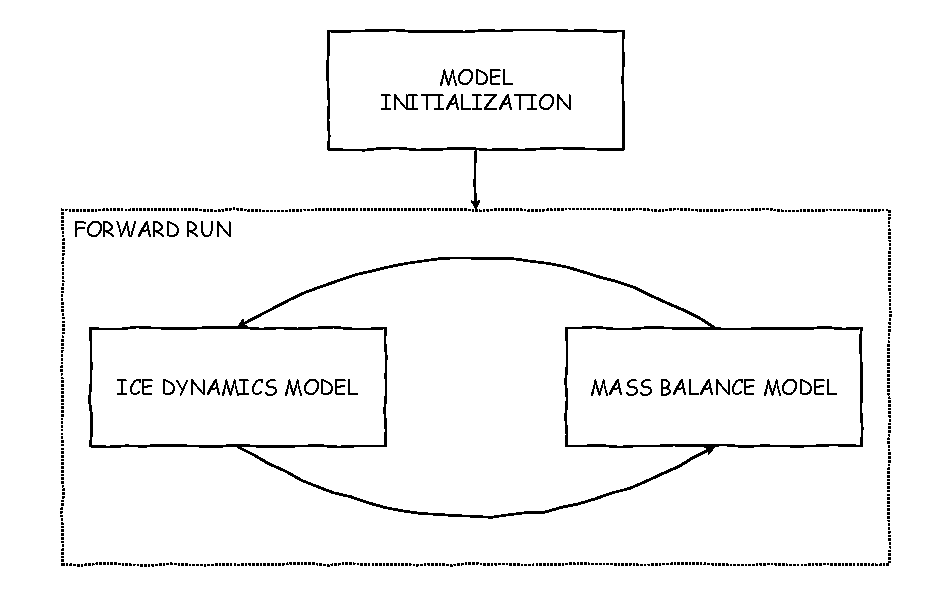
\includegraphics[width=0.65\textwidth]{/Users/oberrauch/work/master/flowchart/model-structure/model-structure.pdf}
    
    \end{frame}
    
    % VAS model initialization on example of HEF
    \begin{frame}[t]\frametitle{Volume/area scaling model initialization}

        \centering
        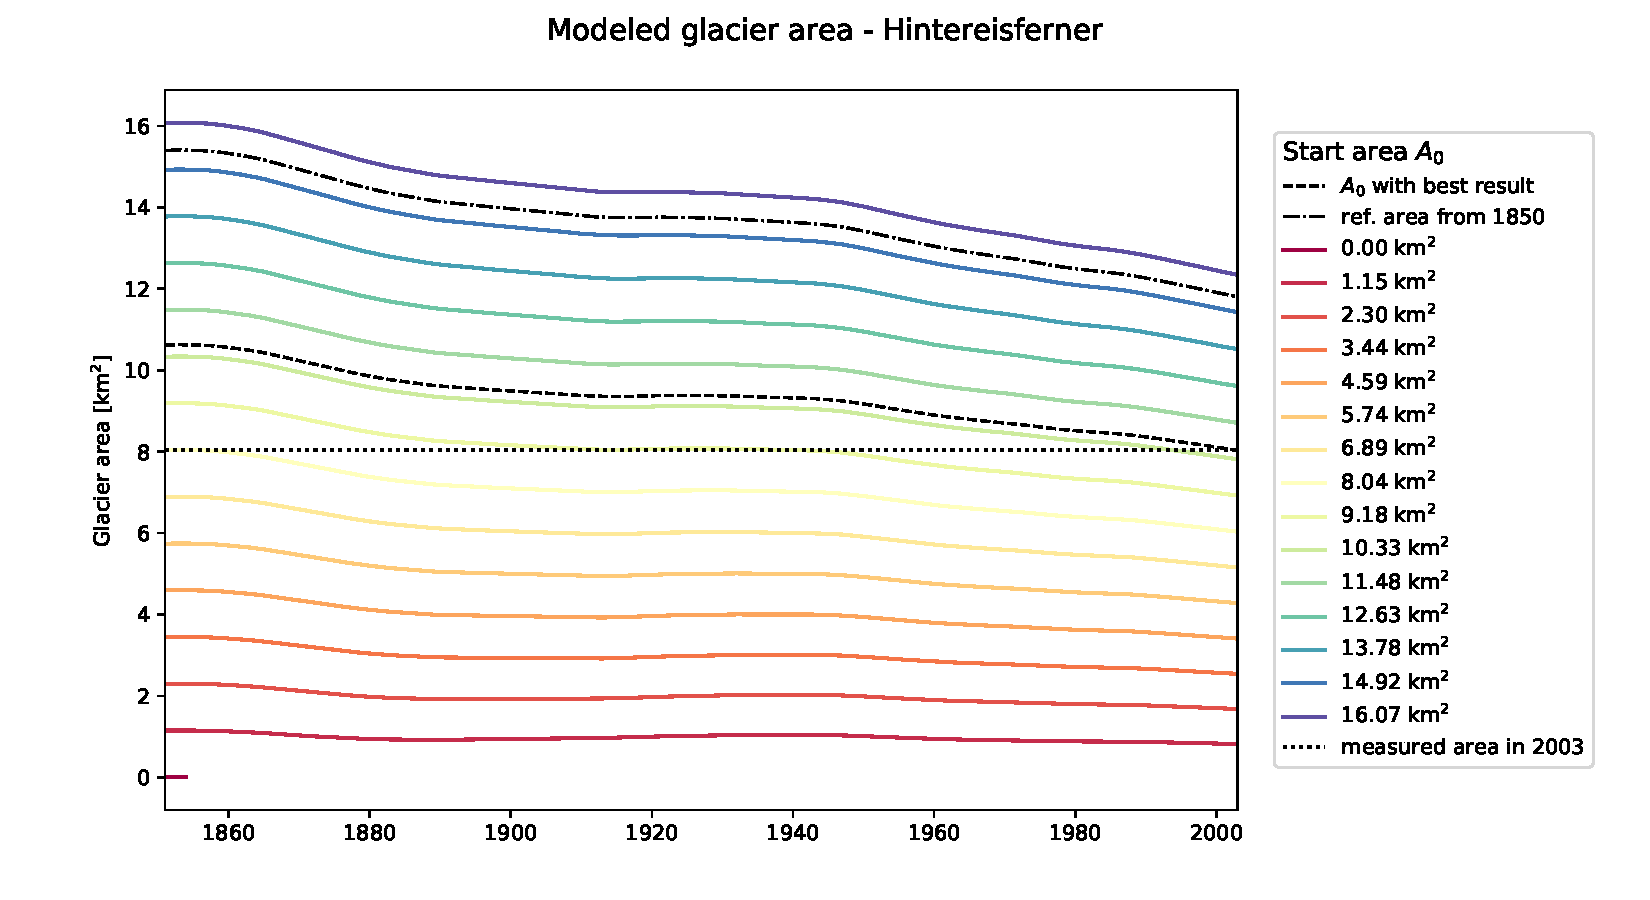
\includegraphics[width=0.9\textwidth]{/Users/oberrauch/Desktop/slides/hintereisferner.jpg}<1>%
        \includegraphics[width=0.9\textwidth]{/Users/oberrauch/Desktop/slides/hintereisferner_outline.pdf}<2>%
        \includegraphics[width=0.9\textwidth]{/Users/oberrauch/Desktop/slides/hintereisferner_area.pdf}<3>%
    
    \end{frame}

    % VAS equations and glacier representation
    \begin{frame}[t]\frametitle{Volume/area scaling model initialization}
        % Volume/area scaling
        \centering
        \vspace*{1cm}
        \only<1-4>{
            Volume/area scaling relation:
            \begin{equation*}
                V = c_A \cdot A^\gamma
            \end{equation*}
        }%
        \only<2-4>{
            \setbeamercovered{transparent}
            \begin{itemize}
                \item<2-> Originally determined as empirical constants, e.g., \citet{Chen1990}
                \item<3-> Physical basis and derivation by \citet{Bahr1997a,Bahr1997b,Bahr2015}
                \item<4> Dimensional analysis, Buckingham-Pi theorem
            \end{itemize}
            
        }
        \only<5->{
            Volume/area scaling relation:
            \begin{equation*}
                V_0 = c_A \cdot {A_0}^\gamma
            \end{equation*}
        }
        % Volume/length scaling
        \only<6->{
            Volume/length scaling relation:
        \begin{equation*}
            V = c_L \cdot {L}^q
        \end{equation*}}
        % Inverted volume/length scaling
        \only<7>{
        Inverted volume/length scaling relation:
        \begin{equation*}
            L_0 = \left(\frac{V_0}{c_L}\right)^{1/q}
        \end{equation*}
        }%
    \end{frame}

    \begin{frame}[t]\frametitle{Volume/area scaling model initialization}
        \centering
        % Glacier as cuboid
        \only<1>{%
        \vfill%
        \includegraphics[width=0.5\textwidth]{/Users/oberrauch/Desktop/slides/cuboid.pdf}}%
        % Cuboid with labels
        \only<2>{%
        \vfill%
        \includegraphics[width=0.5\textwidth]{/Users/oberrauch/Desktop/slides/cuboid_labels.pdf}}%
    \end{frame}

    \begin{frame}[t]\frametitle{Volume/area scaling model initialization}
        \centering
        % Glacier as cuboid
        \only<1>{%
        \vfill%
        \includegraphics[width=0.5\textwidth]{/Users/oberrauch/Desktop/slides/cuboid_elevation.pdf}}%
        % Steep glacier
        \only<2>{%
        \vfill%
        \includegraphics[width=0.5\textwidth]{/Users/oberrauch/Desktop/slides/cuboid_steep.pdf}}%
        % Flat glacier
        \only<3>{%
        \vfill%
        \includegraphics[width=0.5\textwidth]{/Users/oberrauch/Desktop/slides/cuboid_flat.pdf}}%
    
    \end{frame}

    \begin{frame}[c]\frametitle{Model structure}

        \centering
        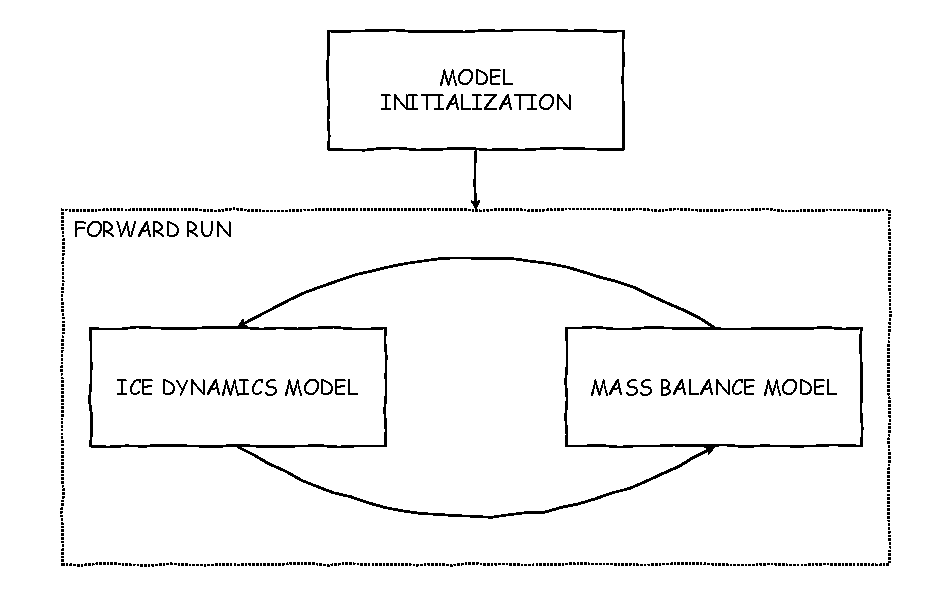
\includegraphics[width=0.65\textwidth]{/Users/oberrauch/work/master/flowchart/model-structure/model-structure.pdf}
    
    \end{frame}

    \begin{frame}[t]\frametitle{Mass balance model}
        
        \centering
        \only<1>{%
        \vfill%
        \includegraphics[width=0.5\textwidth]{/Users/oberrauch/Desktop/slides/cuboid_snow_sun_before.pdf}}%
        \only<2>{%
        \vfill%
        \includegraphics[width=0.5\textwidth]{/Users/oberrauch/Desktop/slides/cuboid_snow_sun.pdf}}%
        % Mass balance equation
        \only<3>{%
            \vfill
            Specific mass balance [\si{\milli\meter\waterequivalent\per\year}] equation from \citet{Marzeion2012b}
            \vspace{0.5cm}
            \begin{equation*}
                B = \left[\sum_{i=1}^{12}\left[
                    P_i^\text{solid}  - \mu^* \cdot \max\left(T_{i}^\text{terminus} - T_\text{melt},\ 0\right)
                \right]\right] - \beta^*
            \end{equation*}
        }%
    
    \end{frame}
    \begin{frame}[t]\frametitle{Mass balance model}
        
        \centering
        \begin{align*}
            T_i^\text{terminus} &= T_i \cdot \gamma_\text{temp} (z_\text{min} - z_\text{ref})\\
            T_{i}^\text{max} &= T_i \cdot \gamma_\text{temp} (z_\text{max} - z_\text{ref})
        \end{align*}
        \begin{align*}
            P_i^\text{solid} = a \cdot P_i \cdot f_\text{solid} \cdot (1 + \gamma_\text{precip} \cdot (z_\text{mean} - z_\text{ref}))
        \end{align*}
        \begin{align*}
            f_\text{solid} = 
                \begin{cases}
                    0   \quad & T_{i}^\text{max} > T_\text{liquid}\\
                    1 + \frac{T_{i}^\text{terminus} - T^\text{solid}}{\gamma_\text{temp}\cdot(z_\text{max} - z_\text{min})} \quad \forall & \text{other}\\
                    1   \quad & T_{i}^\text{terminus} < T_\text{solid} \\
                \end{cases}
        \end{align*}
        
    \end{frame}

    \begin{frame}[c]\frametitle{Model structure}

        \centering
        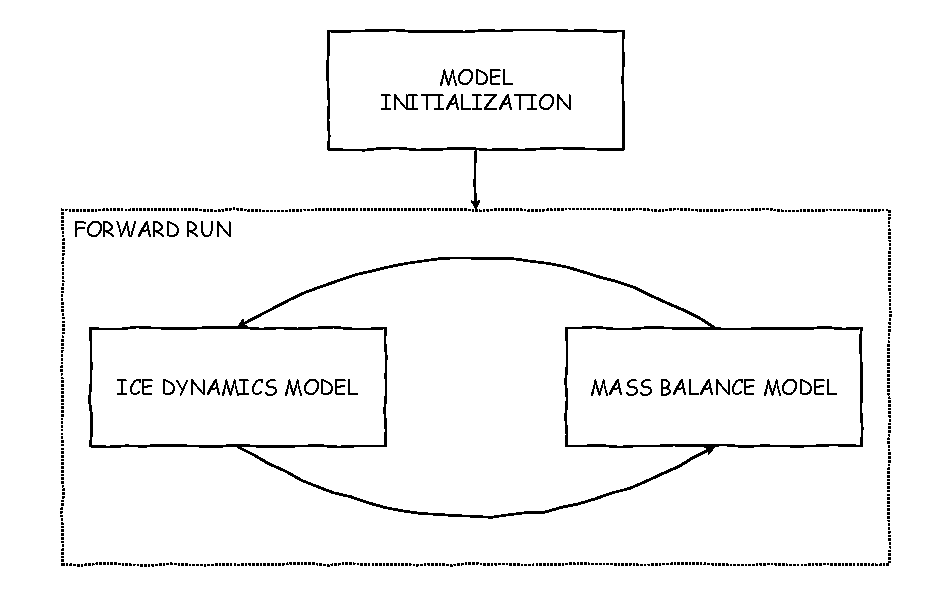
\includegraphics[width=0.65\textwidth]{/Users/oberrauch/work/master/flowchart/model-structure/model-structure.pdf}
    
    \end{frame}

    % Confusogram off the day
    \begin{frame}[c]\frametitle{Model iteration structure}
        
        \centering
        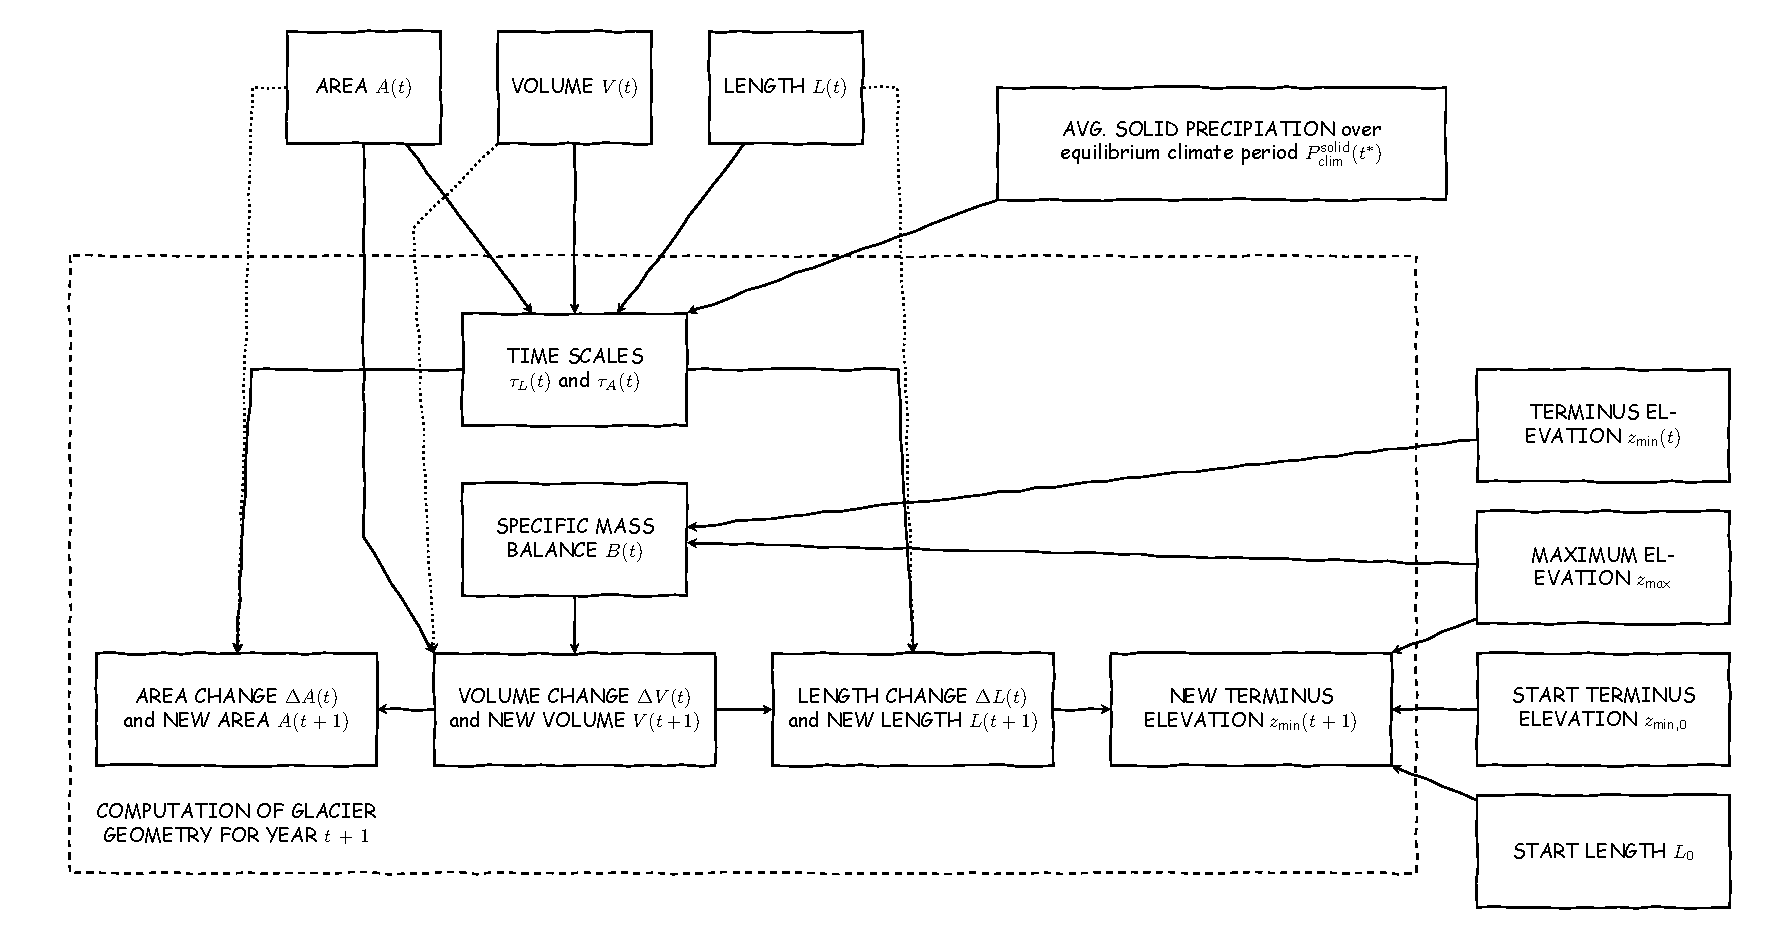
\includegraphics[width=0.95\textwidth]{/Users/oberrauch/work/master/flowchart/iteration-presentation/scaling.pdf}
    
    \end{frame}

    \begin{frame}[t]\frametitle{Volume change}
        \centering
        \only<1,2>{%
            \begin{align*}
                \Delta V(t) = \frac{1}{\rho_\text{ice}} A(t)\cdot B(t)
            \end{align*}
        }%
        \only<2>{%
            \vfill
            Volume changes instantenously
            \begin{align*}
                V(t+1) = V(t) + \Delta V(t)
            \end{align*}
        }%
        \only<3>{%
        \vfill%
        \includegraphics[width=0.5\textwidth]{/Users/oberrauch/Desktop/slides/cuboid_volume_change.pdf}}%
    
    \end{frame}

    \begin{frame}[t]\frametitle{Change of area and length}
        
        \centering
        \vfill%
        \includegraphics[width=0.5\textwidth]{/Users/oberrauch/Desktop/slides/cuboid_area_length_change.pdf}
    
    \end{frame}

    \begin{frame}[t]\frametitle{Response time scaling}
        
        \centering
        \vfill
        \onslide<1->{
        Time scale of glacier length change based on \citet{Johannesson1989}
        \begin{align*}
            \tau_L = \frac{V(t)}{P^\text{solid}_\text{clim}(t^*)A(t)}
        \end{align*}}
        \vfill
        \onslide<2->{
        Time scale of glacier area change assuming instantenous width change
        \begin{align*}
            \tau_A = \tau_L(t)\frac{W(t)}{L(t)} = \tau_L(t)\frac{A(t)}{L(t)^2}
        \end{align*}}
    
    \end{frame}

    % \begin{frame}[t]\frametitle{Change of area and length}
    %     \centering%
    %     \vfill%
    %     \onslide<1->{%
    %         Volume/area scaling relation%
    %         \begin{equation*}%
    %             V = c_A \cdot A^\gamma%
    %         \end{equation*}%
    %     }%
    %     \onslide<2->{%
    %         Inverted volume/area scaling relation%
    %         \begin{equation*}%
    %             A = \left(\frac{V}{c_A}\right)^{1/\gamma}%
    %         \end{equation*}%
    %     }%
    %     \onslide<3->{
    %         Equilibrium changes%
    %         \begin{align*}%
    %             A_\text{eq} = \left(\frac{V(t+1)}{c_A}\right)^{1/\gamma}%
    %         \end{align*}%
    %     }%

    % \end{frame}

    \begin{frame}[t]\frametitle{Change of area and length}

        \centering%
        \vfill%
        \onslide<1->{%
        Equilibrium changes%
        \begin{align*}%
            A_\text{eq} = \left(\frac{V(t+1)}{c_A}\right)^{1/\gamma}%
        \end{align*}}\\[6pt]%
        \onslide<2->{%
        Area changes follow \textbf{response time scaling}:%
        \begin{align*}%
            \Delta A(t) = \frac{1}{\tau_A}\left(\left(\frac{V(t+1)}{c_A}\right)^{1/\gamma} - A(t) \right)%
        \end{align*}}%
        \onslide<3->{%
        \begin{align*}%
            A(t+1) = A(t) + \Delta A(t)%
        \end{align*}}%
    \end{frame}

    \begin{frame}[t]\frametitle{Change of area and length}
        \centering%
        \vfill%
        \onslide<1->{%
        Equilibrium changes%
        \begin{align*}%
            L_\text{eq} = \left(\frac{V(t+1)}{c_L}\right)^{1/q}%
        \end{align*}}\\[6pt]%
        \onslide<1->{%
        Length changes follow \textbf{response time scaling}:%
        \begin{align*}%
            \Delta L(t) = \frac{1}{\tau_L}\left(\left(\frac{V(t+1)}{c_L}\right)^{1/q} - L(t) \right)%
        \end{align*}}%
        \onslide<1->{%
        \begin{align*}%
            L(t+1) = L(t) + \Delta L(t)%
        \end{align*}}%
    \end{frame}

    % Confusogram off the day
    \begin{frame}[t]\frametitle{Change of terminus elevation}
        
        \centering
        \only<1>{
            \vfill
            \includegraphics[width=0.5\textwidth]{/Users/oberrauch/Desktop/slides/cuboid_terminus_elevation_change.pdf}
        }
        \only<2->{
            \vspace{1cm}
            Average (initial) gradient
            \begin{align*}
                \frac{z_\text{min,0} - z_\text{max}}{L_0}
            \end{align*}
        }
        \only<3->{
            Terminus elevation as linear function of glacier length
            \begin{align*}
                z_\text{min}(t+1) = z_\text{max} + L(t+1)\frac{z_\text{min,0} - z_\text{max}}{L_0}
            \end{align*}
        }
        \only<4>{
            {\large\color[HTML]{f69d0e}{Only feedback between glacier geometry and specific  mass balance}}
        }
    
    \end{frame}

    % Confusogram off the day
    \begin{frame}[t]\frametitle{Model iteration structure}
        
        \centering
        \only<1>{%
        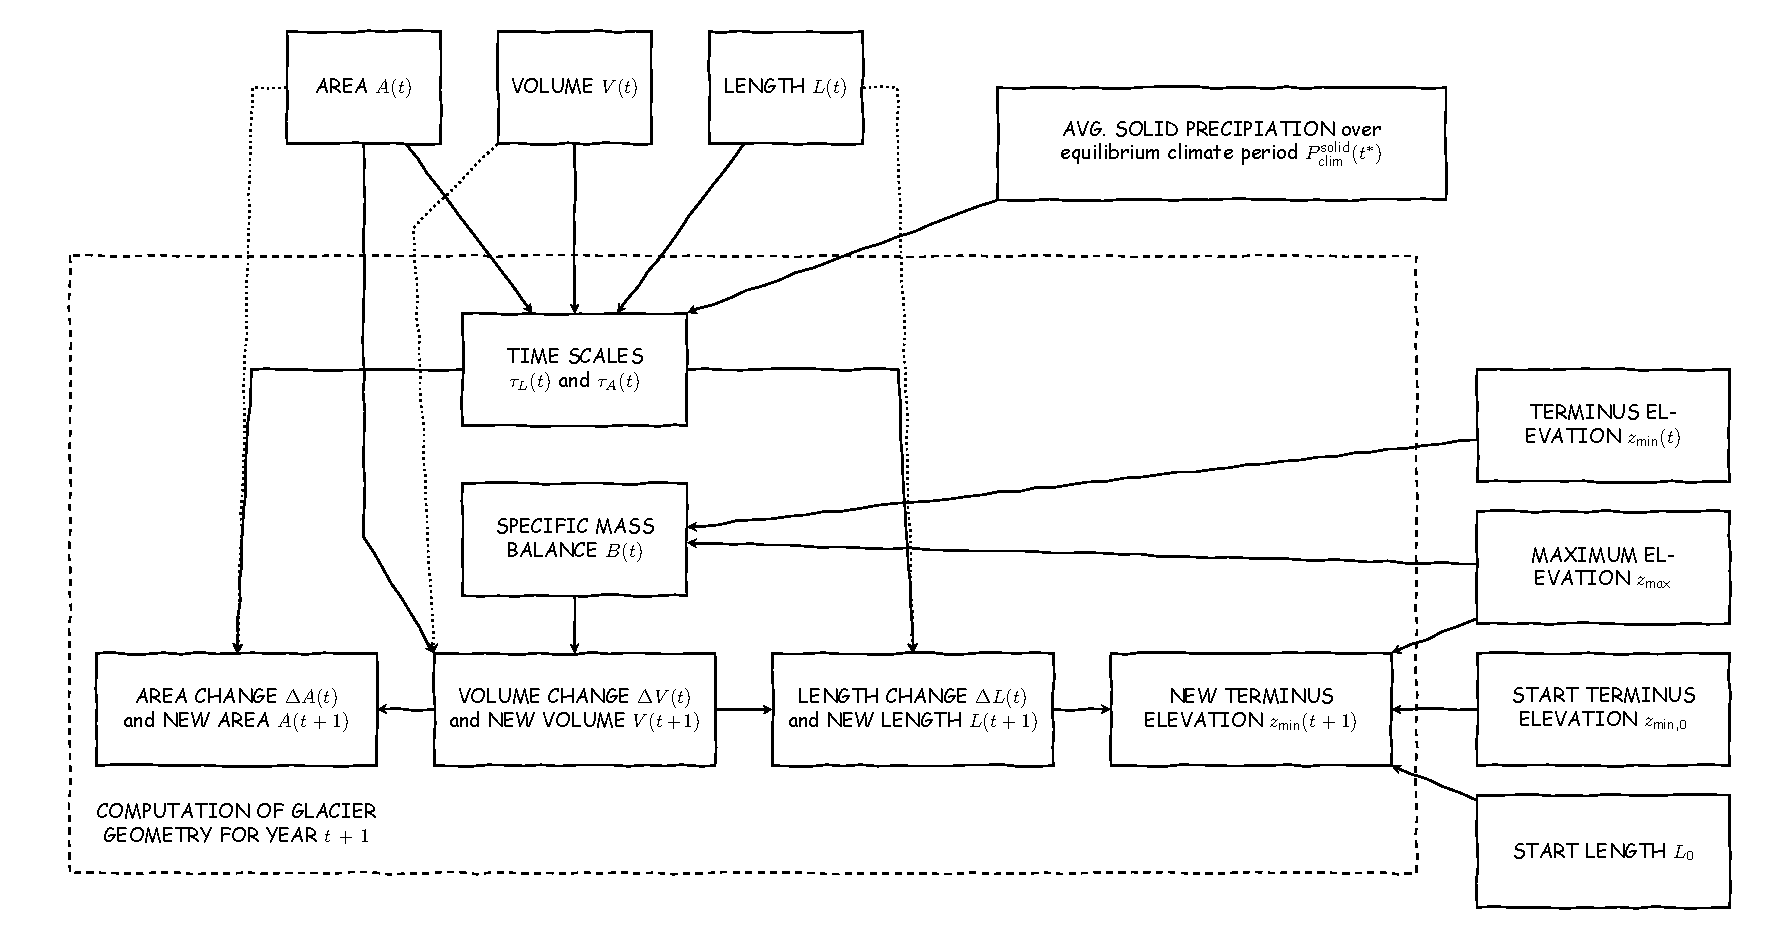
\includegraphics[width=0.95\textwidth]{/Users/oberrauch/work/master/flowchart/iteration-presentation/scaling.pdf}}%
        \only<2>{%
        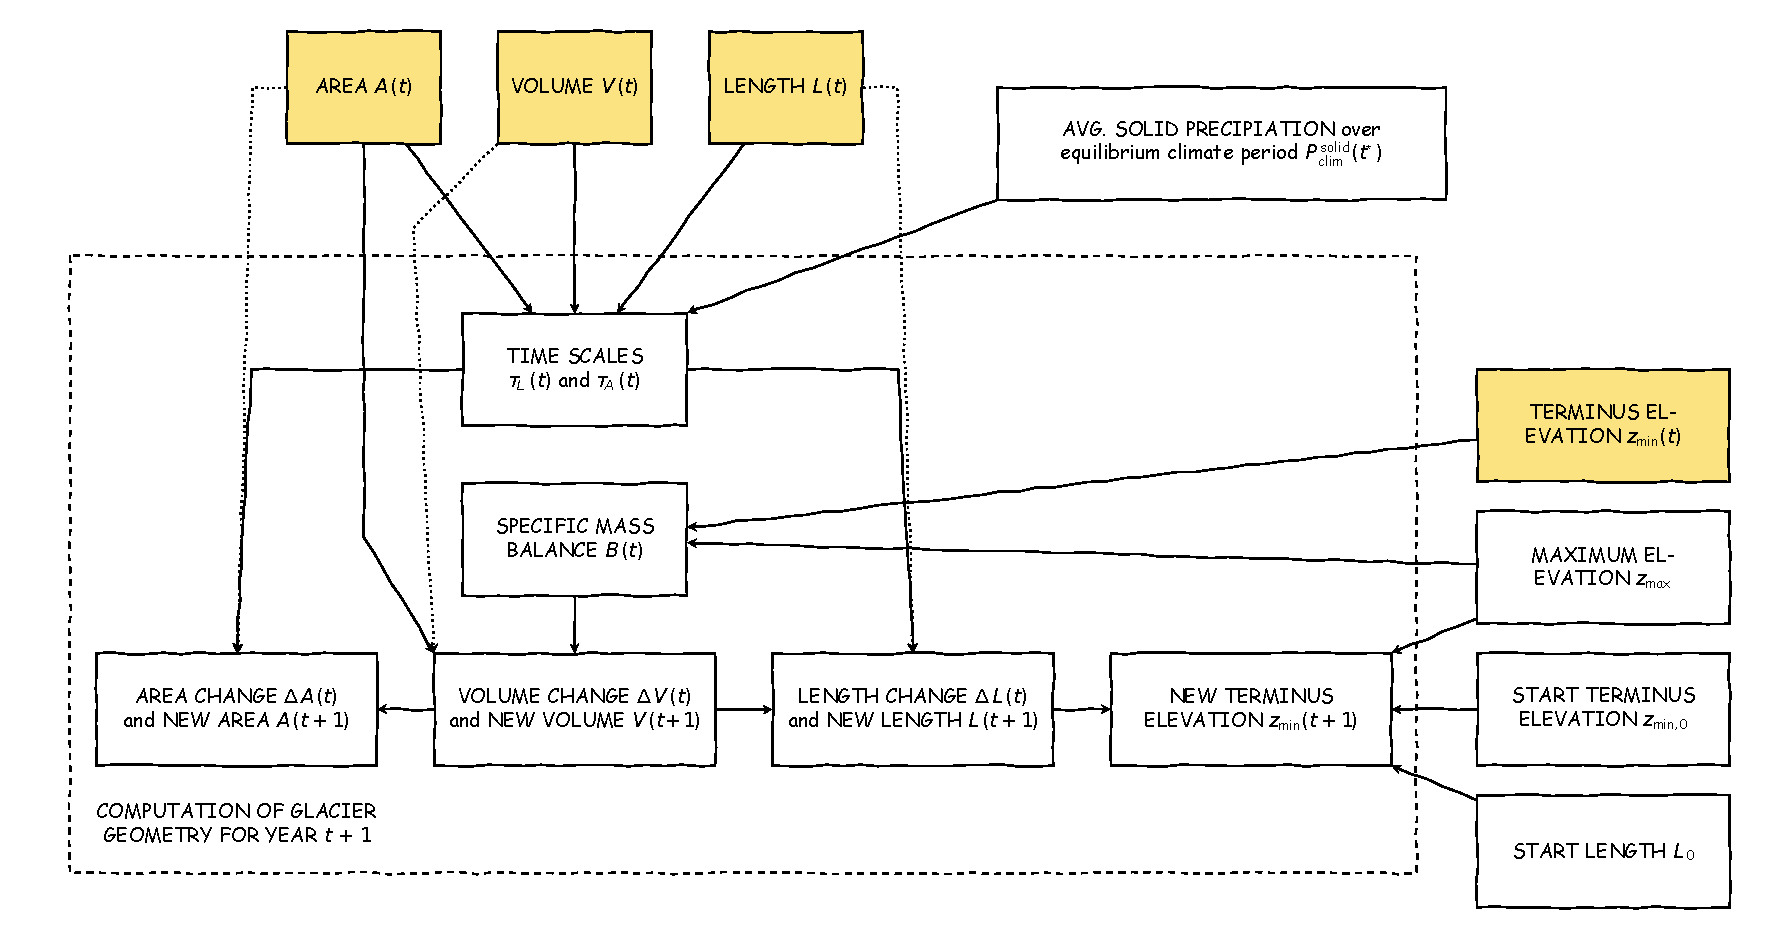
\includegraphics[width=0.95\textwidth]{/Users/oberrauch/work/master/flowchart/iteration-presentation/scaling_t.pdf}}%
        \only<3>{%
        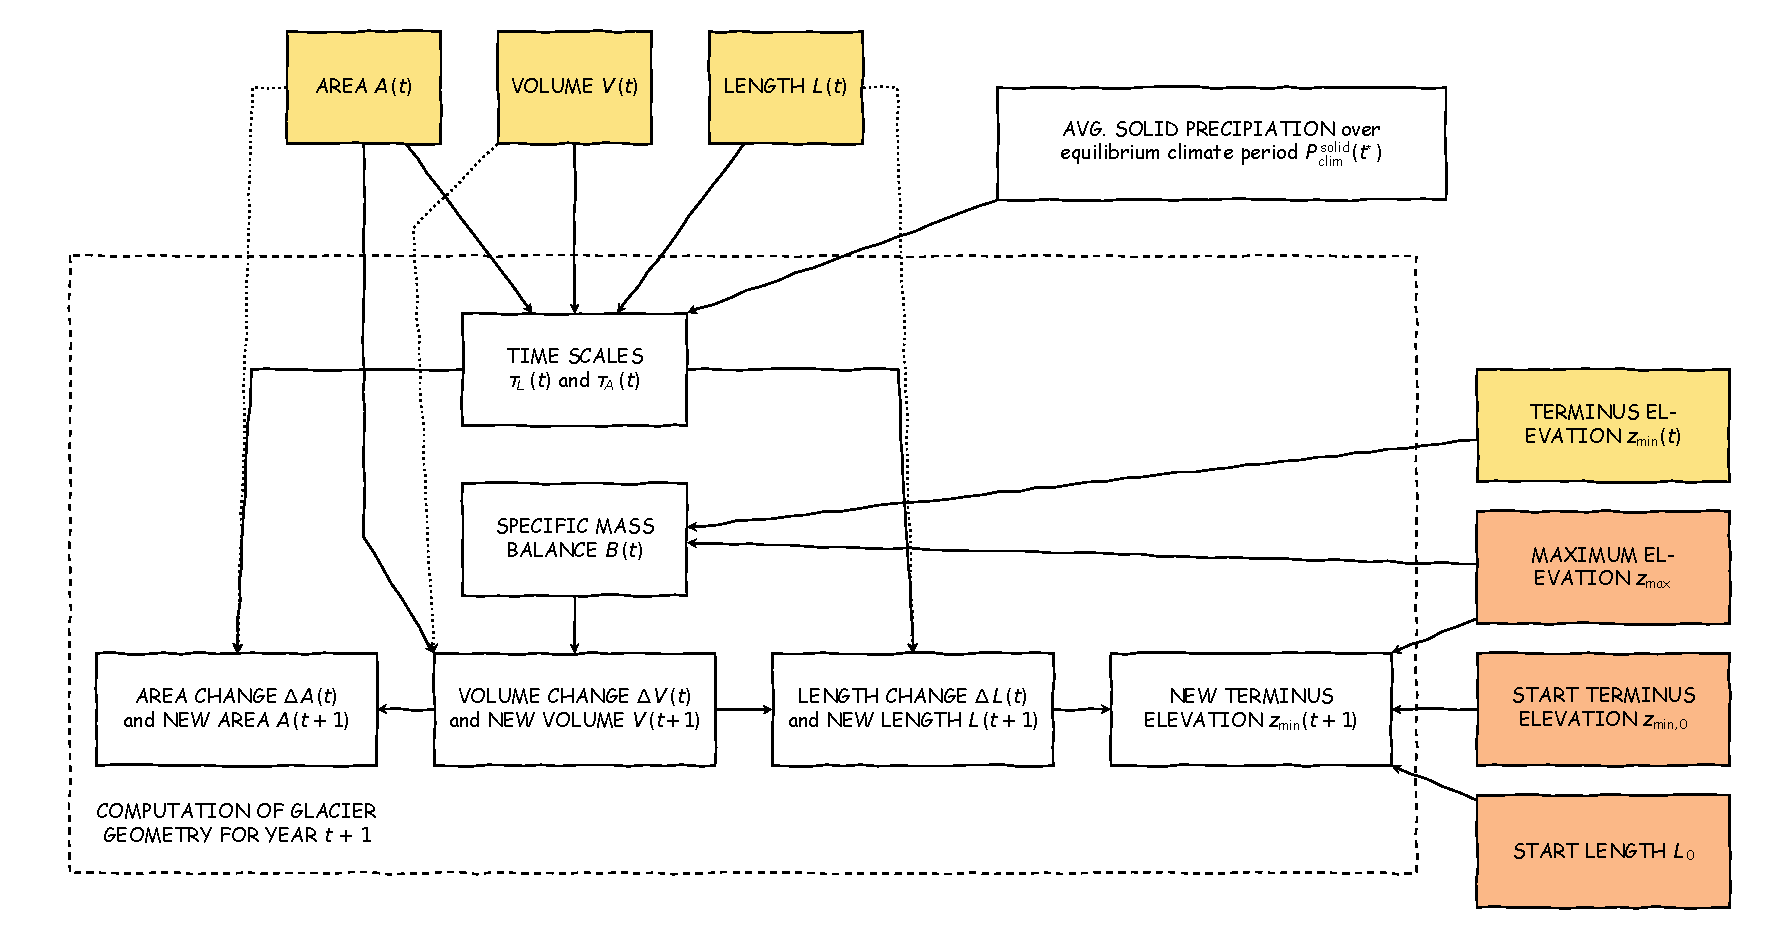
\includegraphics[width=0.95\textwidth]{/Users/oberrauch/work/master/flowchart/iteration-presentation/scaling_t_const.pdf}}%
        \only<4>{%
        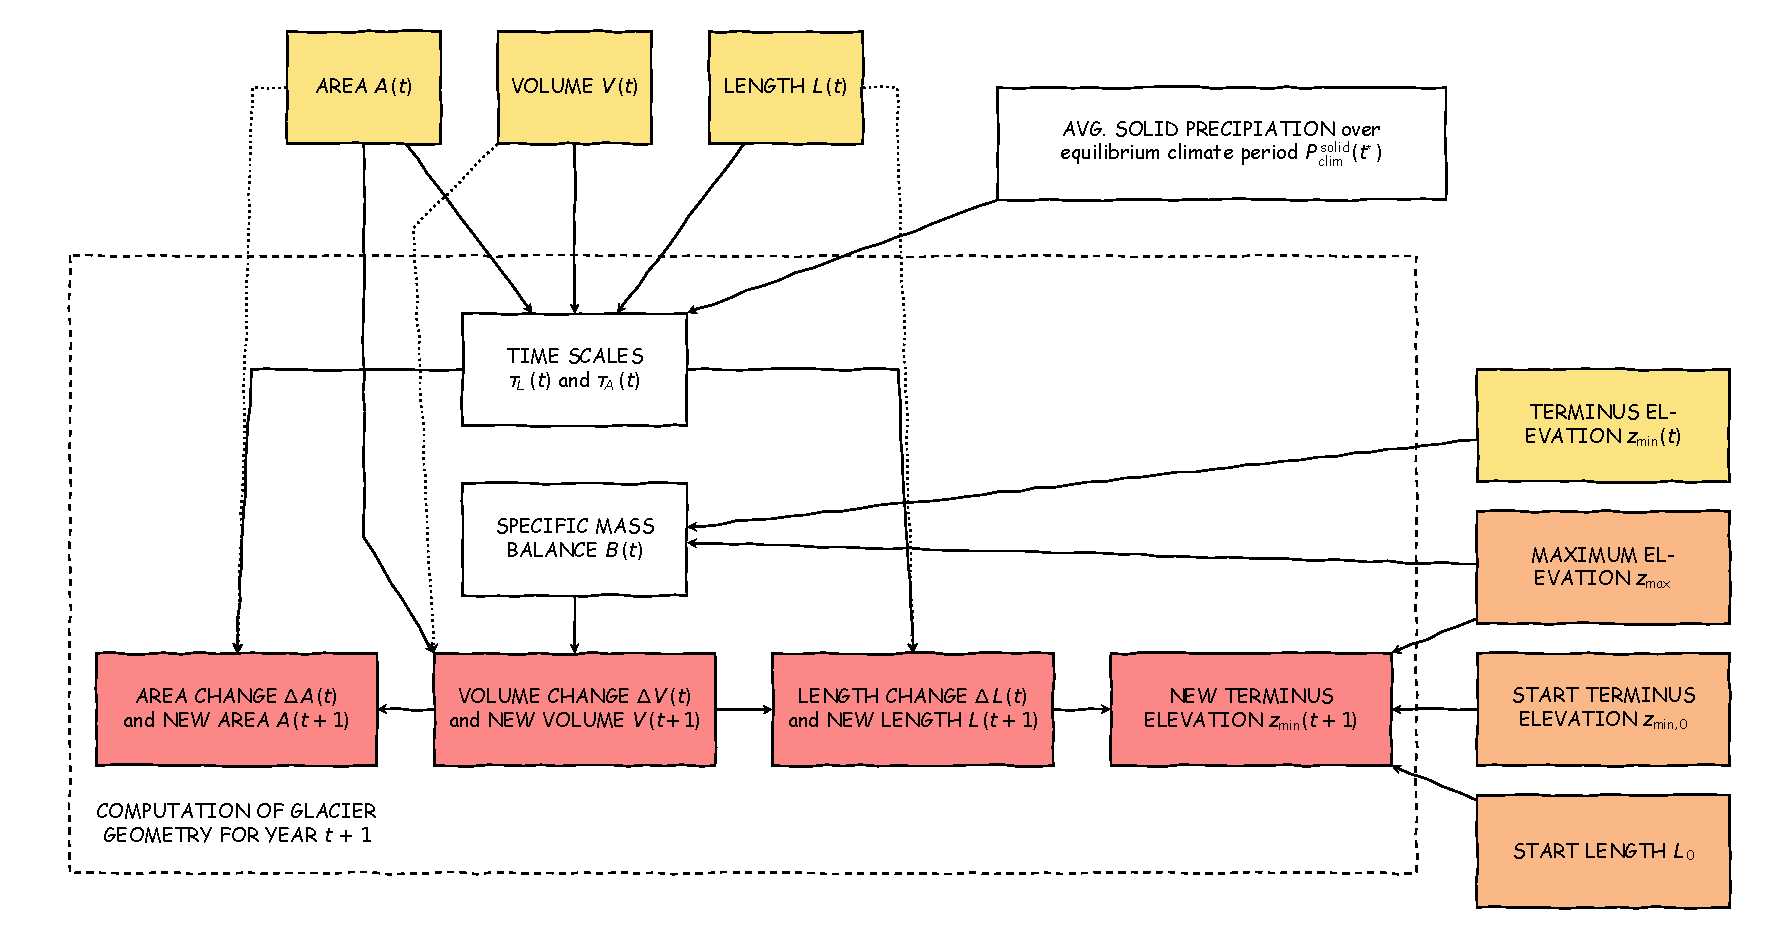
\includegraphics[width=0.95\textwidth]{/Users/oberrauch/work/master/flowchart/iteration-presentation/scaling_t+1.pdf}}%
        
    
    \end{frame}
    
% section vas_model (end)

\section{Flowline model} % (fold)
\label{sec:flowline_model}
    
    \begin{frame}[c]\frametitle{Flowline model}
        
        \centering
        \only<1>{%
        \includegraphics[width=0.7\textwidth]{/Users/oberrauch/Desktop/slides/oggm_logo.png}\\%
        \small{\citet{Maussion2019}, documation under \url{http://docs.oggm.org}}}%
        \only<2>{%
        \includegraphics[width=0.6\textwidth]{/Users/oberrauch/Desktop/slides/hef_flowlines.png}\\
        \footnotesize{Definition of centerlines/flowlines following \citet{Kienholz2014}\\Image source: \url{http://docs.oggm.org}}}%
        \only<3>{%
        \includegraphics[width=0.6\textwidth]{/Users/oberrauch/Desktop/slides/hef_widths.png}\\
        \footnotesize{Flowline width\\Image source: \url{http://docs.oggm.org}}}%
        \only<4>{%
        \includegraphics[width=0.6\textwidth]{/Users/oberrauch/Desktop/slides/hef_widths_corr.png}\\
        \footnotesize{Flowline width corrections\\Image source: \url{http://docs.oggm.org}}}%
        \only<5>{%
        \includegraphics[width=0.6\textwidth]{/Users/oberrauch/Desktop/slides/hef_thickness.png}\\
        \footnotesize{Ice thickness inversion based on \citet{Farinotti2009}\\Image source: \url{http://docs.oggm.org}}}%
        \only<6>{%
        \includegraphics[width=0.9\textwidth]{/Users/oberrauch/Desktop/slides/hintereisferner_flowline.pdf}}%

    \end{frame}

    % Flowline model initialization
    
    % \begin{frame}[c]\frametitle{Flowline model}
        
    %     \centering
    %     \only<1>{%
    %     \includegraphics[width=0.7\textwidth]{/Users/oberrauch/Desktop/slides/oggm_logo.png}\\%
    %     \small{\citet{Maussion2019}, documation under \url{http://docs.oggm.org}}}%
    %     \only<2>{%
    %     \includegraphics[width=0.65\textwidth]{/Users/oberrauch/Desktop/slides/hef_flowlines.png}\\
    %     \footnotesize{Image source: \url{http://docs.oggm.org}}}%
    %     \only<3>{%
    %     \includegraphics[width=0.65\textwidth]{/Users/oberrauch/Desktop/slides/hef_width.png}\\
    %     \footnotesize{Image source: \url{http://docs.oggm.org}}}%
    %     \only<4>{%
    %     \includegraphics[width=0.9\textwidth]{/Users/oberrauch/Desktop/slides/hintereisferner_flowline.pdf}}%

    % \end{frame}


    \begin{frame}[t]\frametitle{Shallow Ice Equations}
        \centering
        \vfill%
        {\renewcommand{\arraystretch}{2}
        \begin{tabular}{lcl}
            \onslide<1->{Volume conservation & \phantom{a} & $\displaystyle \dpar{S}{t} = w\dot b - \nabla\cdot q$}\\
            \onslide<2->{Ice flux & & $\displaystyle q = uS$}\\
            \onslide<3->{Ice velocity & & $\displaystyle u = f_dh\tau^n + f_s\frac{\tau^n}{h}$}\\
            \onslide<4->{Deformation parameter & & $\displaystyle f_d = \frac{2A}{n+2}$}\\
            \onslide<5->{Basal shear stress & & $\displaystyle \tau \approx \tau_d = \alpha\rho_\text{ice}gh$}
        \end{tabular}}
    
    \end{frame}

% section flowline_model (end)

    \begin{frame}[t]\frametitle{Score board}
        \vspace*{0.5cm}
        \begin{columns}
            \begin{column}{0.49\textwidth}
                \textbf{\large{}Volume/area scaling model}
                \vspace*{0.2cm}
                \begin{itemize}
                    \plusitem<2-> Computationally cheap
                    \minusitem<3-> Uniform (cuboid) geometry
                \end{itemize}
                
            \end{column}
            \begin{column}{0.49\textwidth}
                \textbf{\large{}Flowline model}
                \vspace*{0.2cm}
                \begin{itemize}
                    \minusitem<2-> Computationally expensive
                    \plusitem<3-> Geometry aware (1.5 dimensional)
                \end{itemize}
                
            \end{column}
        
        \end{columns}
        
    
    
    \end{frame}


\section{Single glacier test case} % (fold)
\label{sec:single_glacier_test_case}

    \begin{frame}[t]\frametitle{Single glacier test case}

        \begin{minipage}{0.49\textwidth}
            \vspace*{0.5cm}
            \begin{itemize}
                \itemsep=10pt
                \item<1-> Hintereisferner RGI60-11.00897
                \item<2-> Equilibrium experiments with three temperature biases
                    \begin{itemize}
                        \itemsep=5pt
                        \item Cooling scenario with \SI{-0.5}{\celsius}
                        \item Equilibrium scenario with \SI{0}{\celsius}
                        \item Warming scenario with \SI{+0.5}{\celsius}
                    \end{itemize}
                \item<5-> Two mass balance models
                    \begin{itemize}
                        \itemsep=5pt
                        \item \lstinline`ConstantMassBalance()`
                        \item \lstinline`RandomMassBalance()`
                    \end{itemize}
            \end{itemize}
        \end{minipage}
        \hfill
        \begin{minipage}{0.45\textwidth}
            \begin{figure}
                \only<1,2>{
                    \centering
                    \includegraphics[width=\textwidth]{/Users/oberrauch/Desktop/slides/hef_googlemaps.pdf}
                }%
                \only<3>{
                    \centering
                    \includegraphics[width=\textwidth]{/Users/oberrauch/Desktop/slides/plus_temp.pdf}\\%
                    \footnotesize{Adapted from \url{http://edu.oggm.org}, original author: Fabien Maussion}%
                }%
                \only<4->{
                    \centering
                    \includegraphics[width=\textwidth]{/Users/oberrauch/Desktop/slides/minus_temp.pdf}\\%
                    \footnotesize{Adapted from \url{http://edu.oggm.org}, original author: Fabien Maussion}%
                }%
            \end{figure}
        \end{minipage}
    
    \end{frame}


    \begin{frame}[t]\frametitle{Hintereisferner - relative ice volume}
        \centering
        \vfill
        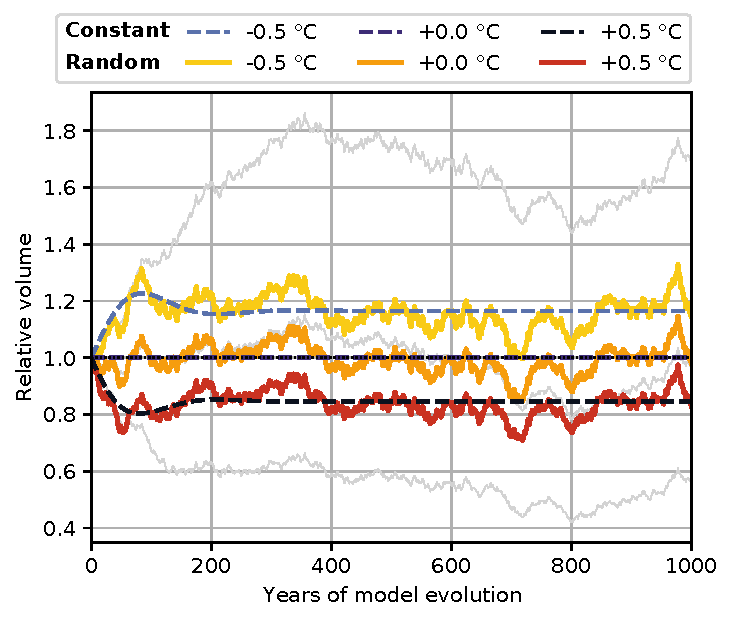
\includegraphics[width=0.49\textwidth]{/Users/oberrauch/Desktop/slides/timeseries/volume_norm_vas_Hintereisferner.pdf}
        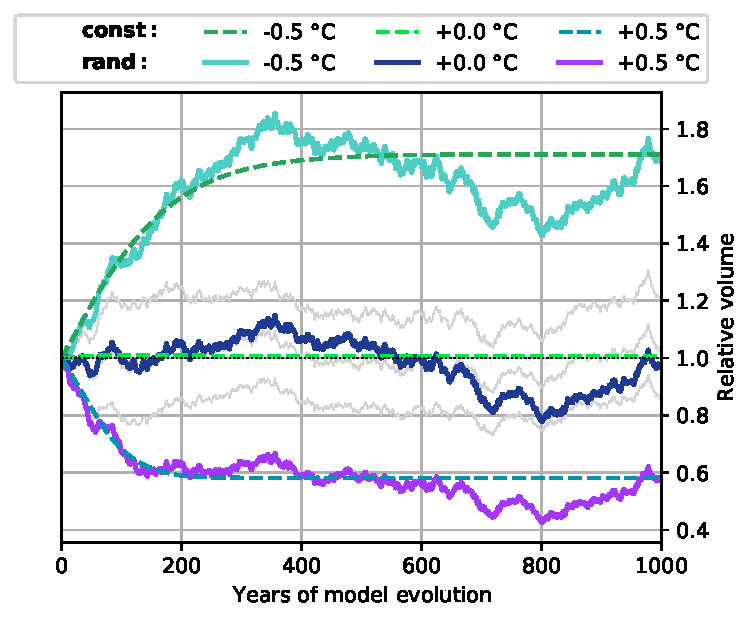
\includegraphics[width=0.49\textwidth]{/Users/oberrauch/Desktop/slides/timeseries/volume_norm_fl_Hintereisferner.pdf}
    \end{frame}
        
    \begin{frame}[t]\frametitle{Hintereisferner - relative surface area}
        \centering
        \vfill
        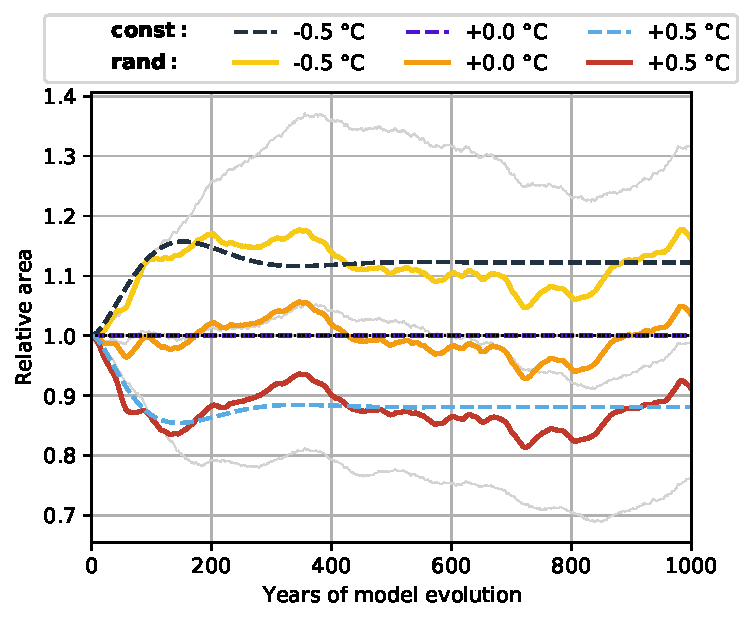
\includegraphics[width=0.49\textwidth]{/Users/oberrauch/Desktop/slides/timeseries/area_norm_vas_Hintereisferner.pdf}
        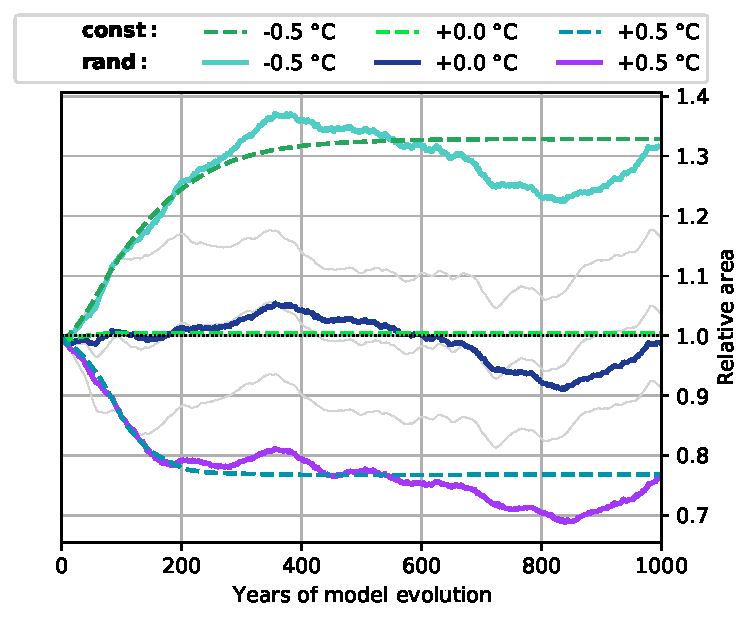
\includegraphics[width=0.49\textwidth]{/Users/oberrauch/Desktop/slides/timeseries/area_norm_fl_Hintereisferner.pdf}
    \end{frame}
        
    \begin{frame}[t]\frametitle{Hintereisferner - relative glacier length}
        \centering
        \vfill
        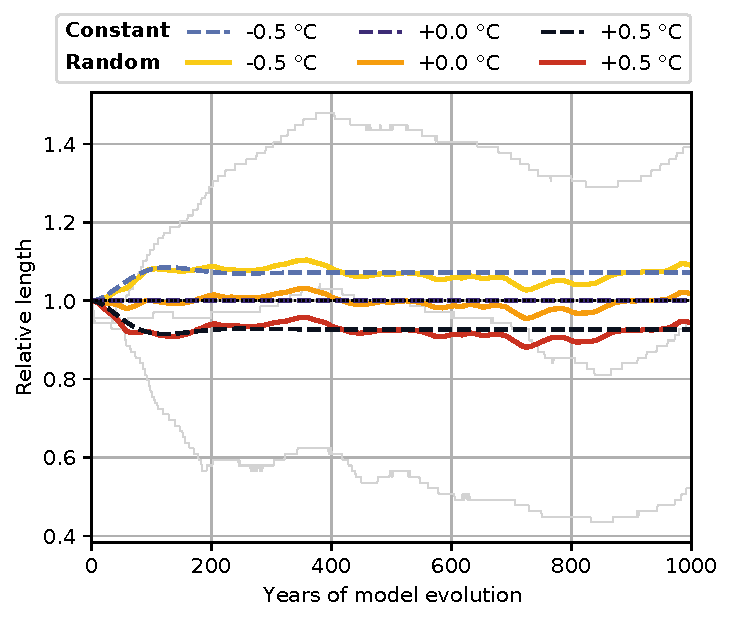
\includegraphics[width=0.49\textwidth]{/Users/oberrauch/Desktop/slides/timeseries/length_norm_vas_Hintereisferner.pdf}
        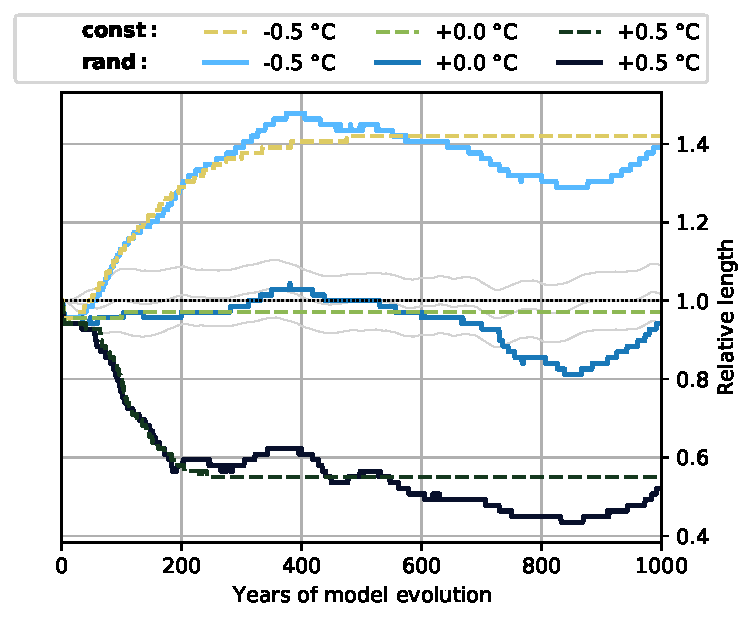
\includegraphics[width=0.49\textwidth]{/Users/oberrauch/Desktop/slides/timeseries/length_norm_fl_Hintereisferner.pdf}
    
    \end{frame}

    \begin{frame}[t]\frametitle{Pasterze - natural length fluctatution}
        \centering
        \vfill
        \includegraphics[width=0.65\textwidth]{/Users/oberrauch/work/master/plots/final_plots/random_length/Pasterze.pdf}
    
    \end{frame}
    
    \begin{frame}[t]\frametitle{Pasterze - power spectral density}
        \centering
        \vfill
        \includegraphics[width=0.65\textwidth]{/Users/oberrauch/work/master/plots/final_plots/psd/Pasterze.pdf}
    
    \end{frame}

    \begin{frame}[t]\frametitle{Pasterze - autocorrelation function}
        \centering
        \vfill
        \includegraphics[width=0.65\textwidth]{/Users/oberrauch/work/master/plots/final_plots/acf/Pasterze.pdf}
    
    \end{frame}

    % Partial autocorrelation function (TODO: move to appendix)
    % \begin{frame}[t]\frametitle{Autocorrelation function}
    %     \centering
    %     \only<1>{HEF - Autocorrelation function:\\[12pt]
    %     \includegraphics[width=0.65\textwidth]{/Users/oberrauch/work/master/plots/final_plots/acf/Hintereisferner.pdf}}
    %     \only<2>{HEF - Partial autocorrelation function:\\[12pt]
    %     \includegraphics[width=0.65\textwidth]{/Users/oberrauch/work/master/plots/final_plots/pacf/Hintereisferner.pdf}}
    
    % \end{frame}%

% section single_glacier_test_case (end)

\section{Regional equilibrium experiments} % (fold)
\label{sec:regional_equilibrium_experiments}

    \begin{frame}[t]\frametitle{HISTALP domain - relative ice volume}
        \centering
        \vfill
        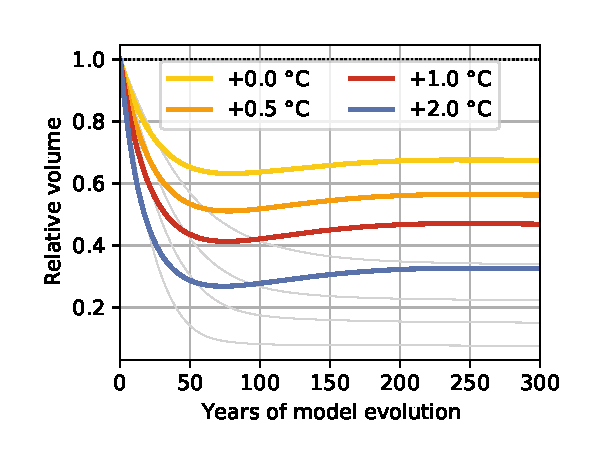
\includegraphics[width=0.49\textwidth]{/Users/oberrauch/work/master/plots/final_plots/time_series/histalp_commitment/volume_norm_vas.pdf}
        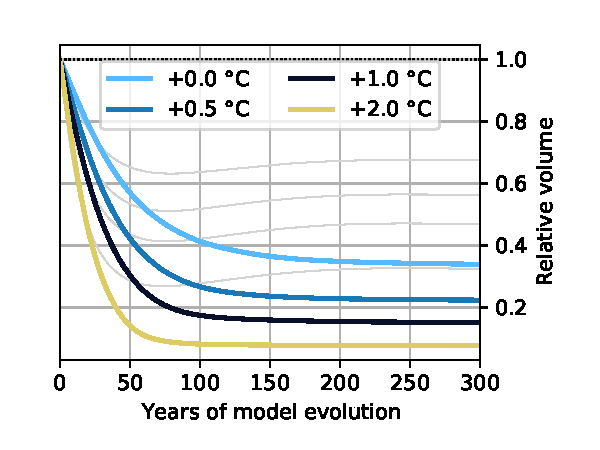
\includegraphics[width=0.49\textwidth]{/Users/oberrauch/work/master/plots/final_plots/time_series/histalp_commitment/volume_norm_fl.pdf}
    \end{frame}

% section regional_equilibrium_experiments (end)

\section{Sensitivity experiments} % (fold)
\label{sec:sensitivity_experiments}

    \begin{frame}[t]\frametitle{Sensitivity experiments}
        \begin{itemize}
            \item TODO.... explain
        \end{itemize}
        

    \end{frame}

    \begin{frame}[t]\frametitle{Sensitivity experiments - Hintereisferner}
        \centering
        \vfill
        \includegraphics[width=0.49\textwidth]{/Users/oberrauch/work/master/plots/final_plots/sensitivity/time_scales_hef.pdf}
        \includegraphics[width=0.49\textwidth]{/Users/oberrauch/work/master/plots/final_plots/sensitivity/scaling_params_hef.pdf}
    \end{frame}

    \begin{frame}[t]\frametitle{Sensitivity experiments - HISTALP domain}
        \centering
        \vfill
        \includegraphics[width=0.49\textwidth]{/Users/oberrauch/work/master/plots/final_plots/sensitivity/time_scales_histalp.pdf}
        \includegraphics[width=0.49\textwidth]{/Users/oberrauch/work/master/plots/final_plots/sensitivity/scaling_params_histalp.pdf}
    \end{frame}

% section sensitivity_experiments (end)

\section{Projections} % (fold)
\label{sec:projections}

    \begin{frame}[t]\frametitle{Projections for the 21st century}
        
        \begin{itemize}
            \item ToDo explain
        \end{itemize}
    
    
    \end{frame}

    \begin{frame}[c]\frametitle{Central Europe - RGI Region 11}
        \centering
        \wider{
            \centering
            \includegraphics[width=0.49\textwidth]{/Users/oberrauch/work/master/plots/final_plots/time_series/cmip/presentation/cmip_vas_11.pdf}
            \includegraphics[width=0.49\textwidth]{/Users/oberrauch/work/master/plots/final_plots/time_series/cmip/presentation/cmip_fl_11.pdf}
        }
    \end{frame}

    \begin{frame}[c]\frametitle{Central Asia - RGI Region 13}
        \centering
        \wider{
            \centering
            \includegraphics[width=0.49\textwidth]{/Users/oberrauch/work/master/plots/final_plots/time_series/cmip/presentation/cmip_vas_13.pdf}
            \includegraphics[width=0.49\textwidth]{/Users/oberrauch/work/master/plots/final_plots/time_series/cmip/presentation/cmip_fl_13.pdf}
        }
    \end{frame}
    

% section projections (end)

\section{Discussion and Conclusion} % (fold)
\label{sec:discussion_and_conclusion}
    \begin{frame}[t]\frametitle{Discussion \& Conclusion}
        
    
    
    \end{frame}

% section discussion_and_conclusion (end)

\appendix
\section{References} % (fold)
\label{sec:references}

    \begin{frame}[t, allowframebreaks]\frametitle{References}
        {\footnotesize
        \bibliographystyle{ametsoc.bst}
        \bibliography{../thesis/master.bib}}
    \end{frame}

\section{Additional slides} % (fold)
\label{sec:additional_slides}
    
    % 21st century projections
    \begin{frame}[c]\frametitle{South Asia West - RGI Region 14}
        \centering
        \wider{
            \centering
            \includegraphics[width=0.49\textwidth]{/Users/oberrauch/work/master/plots/final_plots/time_series/cmip/presentation/cmip_vas_14.pdf}
            \includegraphics[width=0.49\textwidth]{/Users/oberrauch/work/master/plots/final_plots/time_series/cmip/presentation/cmip_fl_14.pdf}
        }
    \end{frame}

    \begin{frame}[c]\frametitle{South Asia East - RGI Region 15}
        \centering
        \wider{
            \centering
            \includegraphics[width=0.49\textwidth]{/Users/oberrauch/work/master/plots/final_plots/time_series/cmip/presentation/cmip_vas_15.pdf}
            \includegraphics[width=0.49\textwidth]{/Users/oberrauch/work/master/plots/final_plots/time_series/cmip/presentation/cmip_fl_15.pdf}
        }
    \end{frame}

% section additional_slides (end)

% section references (end)
	

\end{document}
